\section{Auswertung}
\label{sec:Auswertung}

Die Graphen werden sowohl mit Matplotlib \cite{matplotlib} als auch NumPy \cite{numpy} erstellt. Die Fehlerrechnung wird mithilfe von Uncertainties \cite{uncertainties} durchgeführt.

\subsection{Kalibrierung des Detektors}

Der Detektor wird mit einem $^{152}.{Eu}$-Strahler kalibriert, da dieser ein linienreiches Spektrum für eine möglichst exakte Kalibrierung besitzt.
Für die Kalibrierung wird das $\gamma$-Spektrum der Probe über eine Messdauer von $\SI{2723}{\second}$ aufgenommen. Das Spektrum ist in Abbildung \ref{fig:SpektrumEu} zu sehen. Je eine Ausgleichsrechnung für die einzelnen Energiepeaks der Form
\begin{equation}
N(K)=a \cdot\exp\left(-\frac{1}{2}\left(\frac{K-b}{\sigma}\right)^2\right)+c \label{eq:gaussFit}
\end{equation}
ergibt die Werte in Tabelle \ref{tab:parameterEu}. Der Parameter $a$ gibt dabei die Höhe der Peaks, $b$ die Position und $c$ die Höhe des Untergrundes an. Die Standardabweichung $\sigma$ ist gemäß der Gaußschen Glockenkurve ein Maß für die Breite des Peaks.\\
Den Werten von $b$ werden die entsprechenden Energien aus der Literatur \cite{MARTIN20131497} zugeordnet.
Für die weiteren Ausgleichsrechnungen werden nur die Peaks mit einer Emissionswahrscheinlichkeit über $\SI{2}{\percent}$ berücksichtigt, da der Untergrund die Ergebnisse verfälscht.\\
Die Energieabhängigkeit der Kanäle wird über eine lineare Ausgleichsrechnung der Form
\[
E_\gamma(K) = m\cdot K+n
\]  
bestimmt. Dabei werden die Unsicherheiten der Werte aufgrund ihrer geringen Größe nicht mit berücksichtigt. In Abbildung \ref{fig:Kalibrierung} sind die Energien gegen $K$ aufgetragen.
Für die Parameter ergibt sich:
\begin{align*}
m	&=	\SI{0.402916(21)}{\kilo\electronvolt}\text{,}\\
n	&=	\SI{-3.04(4)}{\kilo\electronvolt}\text{.}
\end{align*}

\begin{figure}
	\centering
	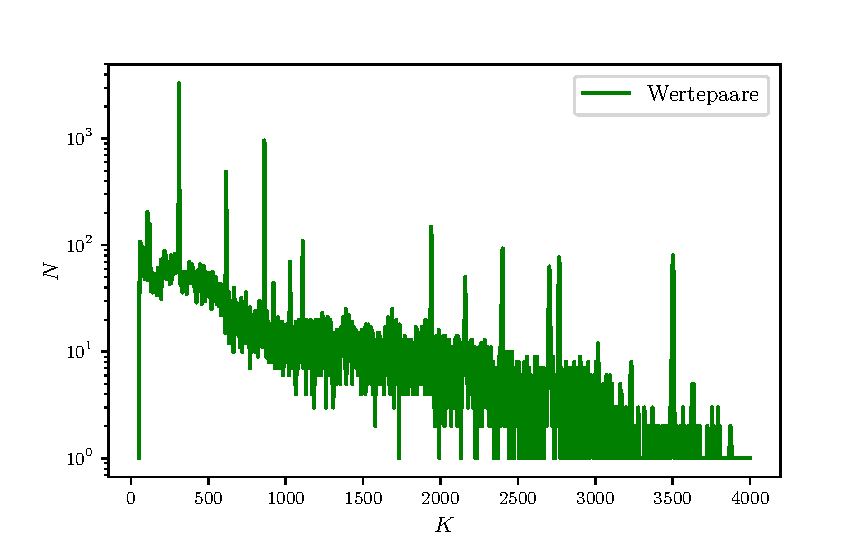
\includegraphics[width=\linewidth-60pt,height=\textheight-60pt,keepaspectratio]{content/images/EU152_1-4000.pdf}
	%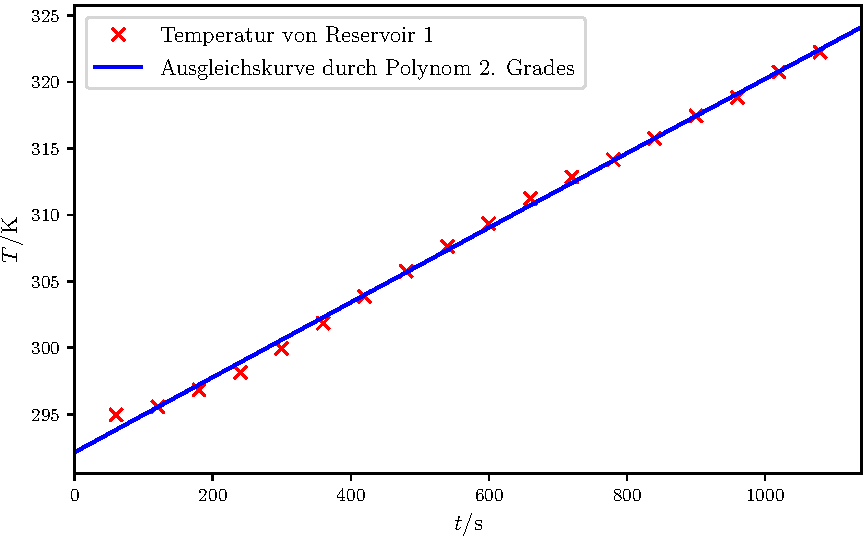
\includegraphics[width=\linewidth-60pt,height=\textheight-60pt,keepaspectratio]{content/images/T1.pdf}
	\caption{Das Spektrum eines $^{152}.{Eu}$-Strahlers, bei einer Messzeit von $\SI{2723}{\second}$, mit der Kanalnummer $K$ und der Anzahl der im Kanal nachgewiesenen Ereignisse $N$.}
	\label{fig:SpektrumEu}
\end{figure}

\begin{table}
	\centering
	\caption{Die Parameter der gefitteten Peaks des Spektrums von $^{152}.{Eu}$ mit den zugeordneten Energien und Wahrscheinlichkeiten aus der Literatur \cite{MARTIN20131497}.}
	\label{tab:a}
	\sisetup{table-format=1.2}
	\begin{tabular}{S[table-format=4.4]@{${}\pm{}$}S[table-format=1.4]S[table-format=2.3]@{${}\pm{}$}S[table-format=1.3]S[table-format=4.3]@{${}\pm{}$}S[table-format=1.3]S[table-format=1.3]@{${}\pm{}$}S[table-format=1.3]S[table-format=4.1]@{${}\pm{}$}S[table-format=2.1]S[table-format=2.2]@{${}\pm{}$}S[table-format=1.2]}
		\toprule
		\multicolumn{2}{c}{$E_\gamma^{\text{lit}}/\si{\kilo\electronvolt}$} & \multicolumn{2}{c}{$W/\si{\percent}$} & \multicolumn{2}{c}{$b$} & \multicolumn{2}{c}{$\sigma$} & \multicolumn{2}{c}{$a$} & \multicolumn{2}{c}{$c$} \\
		\midrule
		121.7817  & 0.0003 & 28.531 & 0.176 & 309.883 & 0.008 & 1.121 & 0.008 & 3213   & 18   & 68   & 6    \\
		244.6974  & 0.0008 & 7.549  & 0.046 & 614.957 & 0.020 & 1.353 & 0.022 & 455    &  6   & 24.5 & 2.0  \\
		295.9387  & 0.0017 & 0.440  & 0.005 & 741.73  & 0.16  & 0.92  & 0.17  & 18.8   & 2.9  & 18.9 & 0.9  \\
		344.2785  & 0.0012 & 26.590 & 0.206 & 862.023 & 0.023 & 1.554 & 0.026 & 970    & 13   & 15   & 6    \\
		367.7891  & 0.0020 & 0.859  & 0.006 & 920.44  & 0.22  & 1.84  & 0.25  & 28     &  4   & 11.2 & 1.3  \\
		411.1165  & 0.0012 & 2.237  & 0.013 & 1027.80 & 0.12  & 1.74  & 0.14  & 59     &  4   & 12.2 & 1.9  \\
		443.9606  & 0.0016 & 2.827  & 0.016 & 1109.51 & 0.09  & 1.72  & 0.10  & 71     &  4   & 10.8 & 1.8  \\
		688.6700  & 0.0050 & 0.856  & 0.007 & 1716.5  & 0.6   & 3.0   & 0.7   &  8.8   & 1.5  & 8.8  & 0.7  \\
		778.9045  & 0.0024 & 12.928 & 0.087 & 1940.48 & 0.06  & 2.10  & 0.07  & 139    &  4   & 10.1 & 1.6  \\
		867.3800  & 0.0030 & 4.228  & 0.032 & 2160.30 & 0.24  & 2.62  & 0.27  & 32.5   & 2.8  & 9.1  & 1.2  \\
		964.0570  & 0.0050 & 14.510 & 0.079 & 2400.01 & 0.10  & 3.04  & 0.11  & 90.3   & 2.6  & 4.6  & 0.8  \\
		1085.8370 & 0.0100 & 10.115 & 0.057 & 2702.63 & 0.24  & 3.37  & 0.27  & 49     &  4   & 5.8  & 1.3  \\
		1112.0760 & 0.0030 & 13.667 & 0.091 & 2767.47 & 0.12  & 3.45  & 0.13  & 69.1   & 2.2  & 2.7  & 0.8  \\
		1212.9480 & 0.0110 & 1.415  & 0.009 & 3017.7  & 0.5   & 3.4   & 0.6   &  7.2   & 1.0  & 1.8  & 0.6  \\
		1299.1420 & 0.0080 & 1.633  & 0.012 & 3232.0  & 0.6   & 4.4   & 0.7   &  4.6   & 0.6  & 0.78 & 0.20 \\
		1408.0130 & 0.0030 & 20.868 & 0.108 & 3502.36 & 0.10  & 4.00  & 0.10  & 74.3   & 1.5  & 0.6  & 0.5  \\
		1457.6430 & 0.0110 & 0.497  & 0.005 & 3629.7  & 0.7   & 6.1   & 0.8   &  3.3   & 0.4  & 0.27 & 0.13 \\
		\bottomrule
	\end{tabular}

	\label{tab:parameterEu}
\end{table}

\begin{figure}
	\centering
	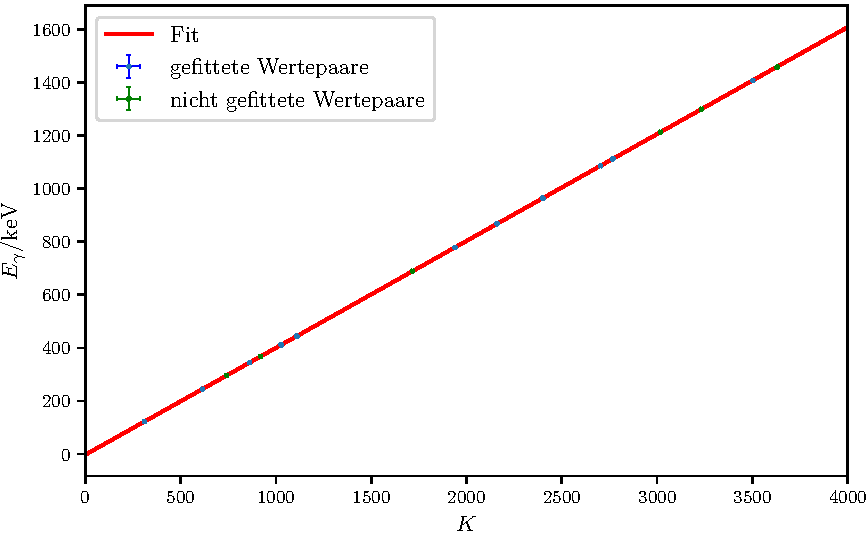
\includegraphics[width=\linewidth-60pt,height=\textheight-60pt,keepaspectratio]{content/images/EnergieKali.pdf}
	\caption{Die Energie $E_\gamma$ gegen die Kanalnummer $K$ aufgetragen, wobei die Unsicherheit des einzelnen Wertepaares sich durch die Unsicherheit der Position der Gaußkurve und der Unsicherheit des Literaturwertes für $E_\gamma$ ergibt.}
	\label{fig:Kalibrierung}
\end{figure}

\subsection{Bestimmung der Effizienz des Detektors}

Zur Bestimmung der Effizienz wird die Vollenergienachweiswahrscheinlichkeit $Q$ berechnet. Dafür müssen die Aktivität $A$, der Raumwinkel $\Omega$, sowie der Inhalt $Z$ der Peaks bestimmt werden.\\
Nach Herstellerangaben beträgt die Aktivität der Probe am 01.10.2000 $\SI{4.13(6)}{\kilo\becquerel}$ und besitzt eine Halbwertszeit von $\SI{4943(5)}{\day}$ \cite{V18}. Betrachtet man die Zeitdifferenz von $\SI{6626(1)}{\day}$ zur Versuchsdurchführung am 21.11.2018, ergibt sich mit Formel \eqref{eq:A} eine aktuelle Aktivität von:
\[
A_.{Eu}=\SI{1.631(24)}{\kilo\becquerel}\text{.}
\]
Der Raumwinkel $\Omega$ bestimmt sich nach Formel \eqref{eq:Omega} zu:
\[
\frac{\Omega}{4\pi} = \num{0.016}
\]
Dabei ist der Radius $r=\SI{2.25}{\centi\metre}$ und der Abstand der Probe zum Detektor ergibt sich zu $a=\SI{8.31}{\centi\metre}$ \cite{V18}.
Der Flächeninhalt $Z$ der Gaußkurven bestimmt sich nach
\begin{equation}
Z = a\sqrt{2\pi\sigma^2} \label{eq:I_Gaus}
\end{equation}
mit den Werten für $a$ und $\sigma$ aus Tabelle \ref{tab:parameterEu}.
Mithilfe von Formel \eqref{eq:Q} und den Literaturwerten für die Wahrscheinlichkeiten \cite{MARTIN20131497} wird $Q$ bestimmt.
Mithilfe der Energiekalibrierung werden die Energien $E_\gamma$ der Peaks über die Kanalnummern bestimmt. Die Ergebnisse sind in Tabelle \ref{tab:Q} eingetragen.\\
In Abbildung \ref{fig:Q} wird $Q$ gegen $E_\gamma$ aufgetragen und es wird eine Ausgleichsrechnung der Form
\[
Q(E_\gamma)=q\cdot \left(\frac{E_\gamma}{\SI{1}{\kilo\electronvolt}}\right)^p
\] 
durchgeführt. Dabei wird zusätzlich der erste Wert nicht mit in die Ausgleichsrechnung mit einbezogen, da hier die Energie unter $\SI{150}{\kilo\electronvolt}$ liegt.  
Es ergeben sich die Parameter:
\begin{align*}
q	&=	\num{81(12)}\text{,}\\
p	&=	\num{-1.025(23)}\text{.}
\end{align*}

\begin{figure}
	\centering
	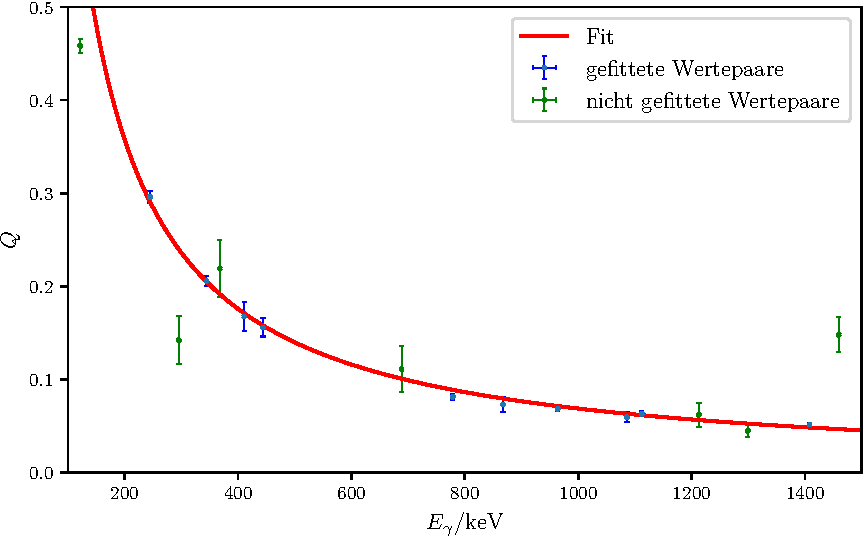
\includegraphics[width=\linewidth-60pt,height=\textheight-60pt,keepaspectratio]{content/images/Q.pdf}
	\caption{Die Vollenergienachweiswahrscheinlichkeit $Q$ gegen die Energie $E_\gamma$ aufgetragen.}
	\label{fig:Q}
\end{figure}

\begin{table}
	\centering
	\caption{Die berechneten Peakinhalte $Z$, die berechneten Vollenergienachweiswahrscheinlichkeiten $Q$, sowie die berechneten Energien $E_\gamma$. Zudem die aus der Literatur entnommenen Energien $E_\gamma^.{lit}$ und Emissions-Wahrscheinlichkeiten $W$ \cite{MARTIN20131497}.}
	\label{tab:a2}
	\sisetup{table-format=1.2}
	\begin{tabular}{S[table-format=4.2]@{${}\pm{}$}S[table-format=1.2]S[table-format=4.4]@{${}\pm{}$}S[table-format=1.4]S[table-format=2.3]@{${}\pm{}$}S[table-format=1.3]S[table-format=4.0]@{${}\pm{}$}S[table-format=2.0]S[table-format=1.4]@{${}\pm{}$}S[table-format=1.4]}
		\toprule
		\multicolumn{2}{c}{$E_\gamma/\si{\kilo\electronvolt}$} & \multicolumn{2}{c}{$E_\gamma^{\text{lit}}/\si{\kilo\electronvolt}$} & \multicolumn{2}{c}{$W/\si{\percent}$} & \multicolumn{2}{c}{$Z$} & \multicolumn{2}{c}{$Q$} \\
		\midrule
		121.82  & 0.04 & 121.7817  & 0.0003 & 28.531 & 0.176 & 9030 & 60 & 0.458  & 0.008  \\
		244.74  & 0.04 & 244.6974  & 0.0008 & 7.549  & 0.046 & 1543 & 25 & 0.296  & 0.007  \\
		295.82  & 0.08 & 295.9387  & 0.0017 & 0.440  & 0.005 &   43 &  8 & 0.142  & 0.026  \\
		344.28  & 0.03 & 344.2785  & 0.0012 & 26.590 & 0.206 & 3780 & 70 & 0.206  & 0.005  \\
		367.82  & 0.10 & 367.7891  & 0.0020 & 0.859  & 0.006 &  130 & 19 & 0.22   & 0.04   \\
		411.08  & 0.06 & 411.1165  & 0.0012 & 2.237  & 0.013 &  259 & 24 & 0.168  & 0.016  \\
		444.00  & 0.05 & 443.9606  & 0.0016 & 2.827  & 0.016 &  304 & 19 & 0.156  & 0.010  \\
		688.56  & 0.22 & 688.6700  & 0.0050 & 0.856  & 0.007 &   66 & 15 & 0.111  & 0.025  \\
		778.81  & 0.03 & 778.9045  & 0.0024 & 12.928 & 0.087 &  727 & 24 & 0.081  & 0.003  \\
		867.38  & 0.10 & 867.3800  & 0.0030 & 4.228  & 0.032 &  213 & 23 & 0.073  & 0.008  \\
		963.96  & 0.05 & 964.0570  & 0.0050 & 14.510 & 0.079 &  687 & 23 & 0.0686 & 0.0026 \\
		1085.89 & 0.11 & 1085.8370 & 0.0100 & 10.115 & 0.057 &  420 & 40 & 0.060 & 0.005  \\
		1112.02 & 0.06 & 1112.0760 & 0.0030 & 13.667 & 0.091 &  597 & 23 & 0.0632 & 0.0026 \\
		1212.85 & 0.19 & 1212.9480 & 0.0110 & 1.415  & 0.009 &   61 & 13 & 0.062  & 0.013 \\
		1299.18 & 0.24 & 1299.1420 & 0.0080 & 1.633  & 0.012 &   51 &  8 & 0.045  & 0.007 \\
		1408.12 & 0.06 & 1408.0130 & 0.0030 & 20.868 & 0.108 &  744 & 17 & 0.0517 & 0.0015 \\
		1459.41 & 0.28 & 1457.6430 & 0.0110 & 0.497  & 0.005 &   51 &  7 & 0.148  & 0.019 \\
		\bottomrule
	\end{tabular}

	\label{tab:Q}
\end{table}

\subsection{Untersuchung des Spektrums von $^{137}.{Cs}$}

Es wird das Spektrum von $^{137}.{Cs}$ bei einer Messzeit von $\SI{4543}{\second}$ aufgenommen. Das Spektrum ist in Abbildung \ref{fig:SpektrumCs} zu sehen. Der Rückstreupeak wird obwohl es sich nicht um einen Gaußpeak handelt wie der Photopeak als Gaußförmig genähert. Das dies eine gute Näherung ist, lässt sich anhand der Fehler in Tabelle \ref{tab:parameterCs} erkennen. Es werden also der Photopeak und der Rückstreupeak mithilfe zweier Ausgleichsrechnungen gemäß Formel \eqref{eq:gaussFit} untersucht. Es ergeben sich die Werte aus Tabelle \ref{tab:parameterCs}. Die Energien bestimmen sich wie zuvor über die Kalibrierung aus dem Parameter $b$.    

\begin{figure}
	\centering
	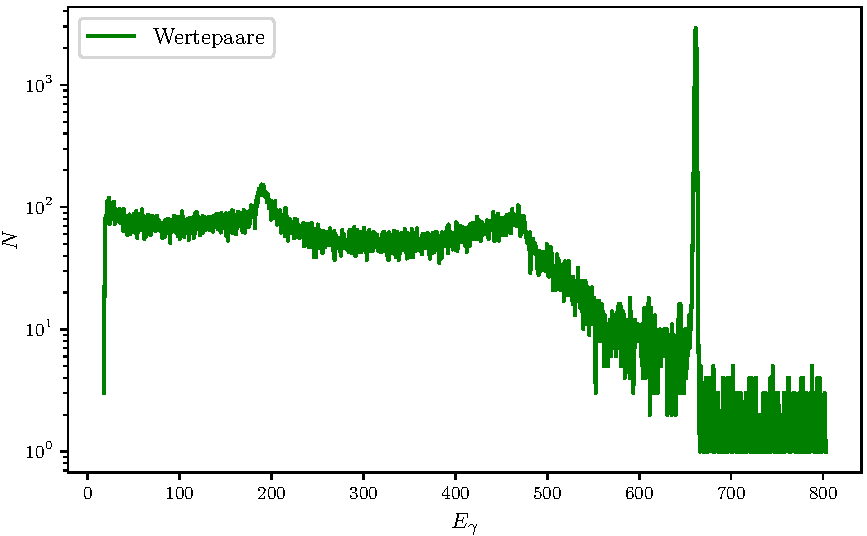
\includegraphics[width=\linewidth-60pt,height=\textheight-60pt,keepaspectratio]{content/images/Cs137.pdf}
	\caption{Das Spektrum eines $^{137}.{Cs}$-Strahlers, bei einer Messzeit von $\SI{4543}{\second}$.}
	\label{fig:SpektrumCs}
\end{figure}

\begin{table}
	\centering
	\caption{Die Parameter der gefitteten Peaks des Spektrums von $^{137}.{Cs}$ mit den ermittelten Energien, wobei es sich beim zweiten Peak um den Rückstreupeak handelt.}
	\label{tab:b}
	\sisetup{table-format=1.2}
	\begin{tabular}{S[table-format=4.2]@{${}\pm{}$}S[table-format=1.2]S[table-format=1.2]@{${}\pm{}$}S[table-format=1.2]S[table-format=4.0]@{${}\pm{}$}S[table-format=2.0]S[table-format=2.1]@{${}\pm{}$}S[table-format=2.1]S[table-format=4.2]@{${}\pm{}$}S[table-format=1.2]}
		\toprule
		\multicolumn{2}{c}{$b$} & \multicolumn{2}{c}{$\sigma$} & \multicolumn{2}{c}{$a$} & \multicolumn{2}{c}{$c$} & \multicolumn{2}{c}{$E_\gamma/\si{\kilo\electronvolt}$} \\
		\midrule
		1649.21 & 0.04 & 2.17  & 0.04 & 2983 & 40 & 20   & 16  & 661.45 & 0.03 \\
		481.2   & 0.7  & 14.5  & 0.8  &   63 &  3 & 77.9 & 1.2 & 190.83 & 0.27 \\
		\bottomrule
	\end{tabular}

	\label{tab:parameterCs}
\end{table}

\noindent Des Weiteren werden die Halbwerts- und die Zehntelwertsbreite des Photopeaks bestimmt. Hierzu werden die linke und die rechte Flanke des Peaks durch Geraden der Form 
\begin{equation}
N(K) = mK+n	\label{eq:Gerade}
\end{equation}
approximiert (vergleiche Abbildung \ref{fig:2tel} und \ref{fig:10tel}). Die Werte sind in Tabelle \ref{tab:geradenBreite} eingetragen, wobei sie von oben nach unten durchnummeriert sind. Mit einer Peakhöhe von $H=2913$ ergeben sich die in Energien umgerechneten Breiten zu:
\begin{align*}
B_{1/2} &= \frac{H/2-n_2}{m_2}-\frac{H/2-n_1}{m_1} \equiv \SI{2.18(4)}{\kilo\electronvolt}\text{,}\\
B_{1/10} &= \frac{H/10-n_4}{m_4}-\frac{H/10-n_3}{m_3} \equiv \SI{4.07(13)}{\kilo\electronvolt}\text{.}
\end{align*}
Dabei ergeben sich die Fehler aus der Gaußschen Fehlerfortpflanzung.
Betrachtet man das Verhältnis der Breiten, so ergibt sich ein Wert von 
\[
\frac{B_{1/10}}{B_{1/2}} = \num{1.87(7)}\text{.}
\]
Dies entspricht dem Wert des Verhältnisses bei einer Gaußkurve von $\num{1.823}$.
Der theoretische Wert für die Halbwertsbreite ergibt sich mit Formel \eqref{eq:dE} zu:
\[
B_{1/2,theo} = \SI{1.031352(19)}{\kilo\electronvolt}\text{.}
\]
Dies entspricht weniger als der Hälfte des experimentellen Wertes.

\begin{figure}
	\centering
	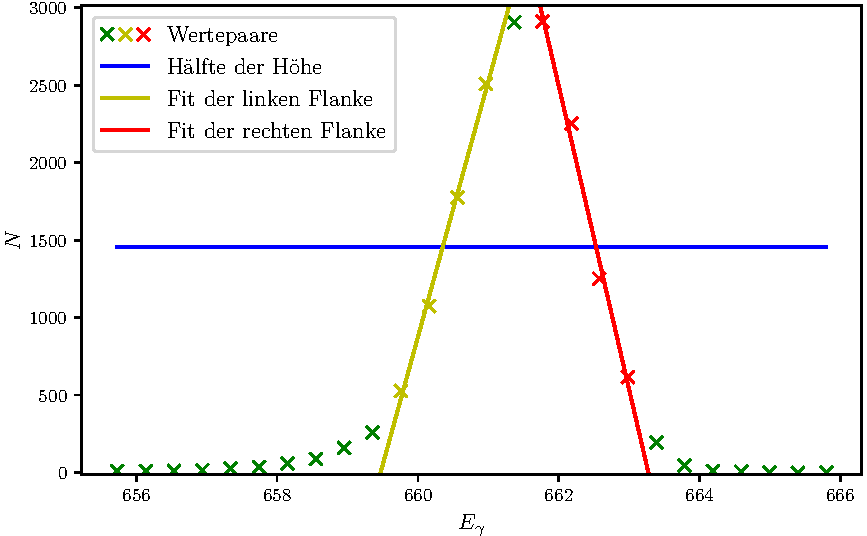
\includegraphics[width=\linewidth-60pt,height=\textheight-60pt,keepaspectratio]{content/images/Cs137Halb.pdf}
	\caption{Die Bestimmung der Halbwertsbreite des $^{137}.{Cs}$-Strahlers. Die gelben Werte werden in die Ausgleichsrechnung der linken Flanke mit einbezogen, die roten in die der Rechten. Die grünen Werte werden in den Ausgleichsrechnungen nicht berücksichtigt.}
	\label{fig:2tel}
\end{figure}

\begin{figure}
	\centering
	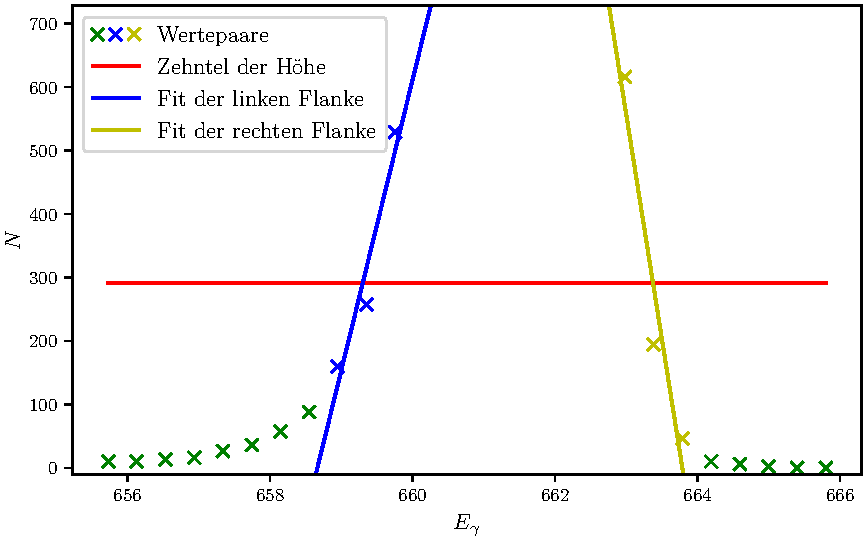
\includegraphics[width=\linewidth-60pt,height=\textheight-60pt,keepaspectratio]{content/images/Cs137Zehntel.pdf}
	\caption{Die Bestimmung der Zehntelwertsbreite des $^{137}.{Cs}$-Strahlers. Die gelben Werte werden in die Ausgleichsrechnung der linken Flanke mit einbezogen, die roten in die der Rechten. Die grünen Werte werden in den Ausgleichsrechnungen nicht berücksichtigt.}
	\label{fig:10tel}
\end{figure}

\begin{table}
	\centering
	\caption{Die Parameter der Ausgleichsgeraden zur Bestimmung der Halbwertsbreite und Zehntelwertsbreite des Vollenergiepeaks des Spektrums von $^{137}.{Cs}$.}
	\label{tab:geraden1}
	\sisetup{table-format=1.2}
	\begin{tabular}{lS[table-format=4.0]@{${}\pm{}$}S[table-format=2.0]S[table-format=8.0]@{${}\pm{}$}S[table-format=6.0]}
		\toprule
		{} & \multicolumn{2}{c}{$m$} & \multicolumn{2}{c}{$n$} \\
		\midrule
		{HWB links}  &  660 & 40 & -1090000 &  60000 \\
		{HWB rechts} & -790 & 60 &  1310000 &  90000 \\
		{ZWB links}  &  190 & 60 &  -300000 &  90000 \\
		{ZWB rechts} & -290 & 80 &   470000 & 130000 \\
		\bottomrule
	\end{tabular}

	\label{tab:geradenBreite}
\end{table}

\newpage
\noindent Als nächstes wird das Compton-Kontinuum untersucht. Die theoretische Lage der Compton-Kante berechnet sich mit der Energie des Photopeaks mit Formel \eqref{eq:Emax} zu:
\[
E_.{Compton,Theo} = \SI{477.147(19)}{\kilo\electronvolt}\text{.}
\]
Der Experimentelle Wert wird über den Schnittpunkt zweier Geraden der Form \eqref{eq:Gerade} bestimmt (vergleiche  Abbildung \ref{fig:Emax}). Mit den Parametern aus Tabelle \ref{tab:geradenEmax} ergibt sich ein Wert von:
\[
E_.{Compton,Exp} = \SI{469.8(10)}{\kilo\electronvolt}\text{.}
\]

\begin{figure}
	\centering
	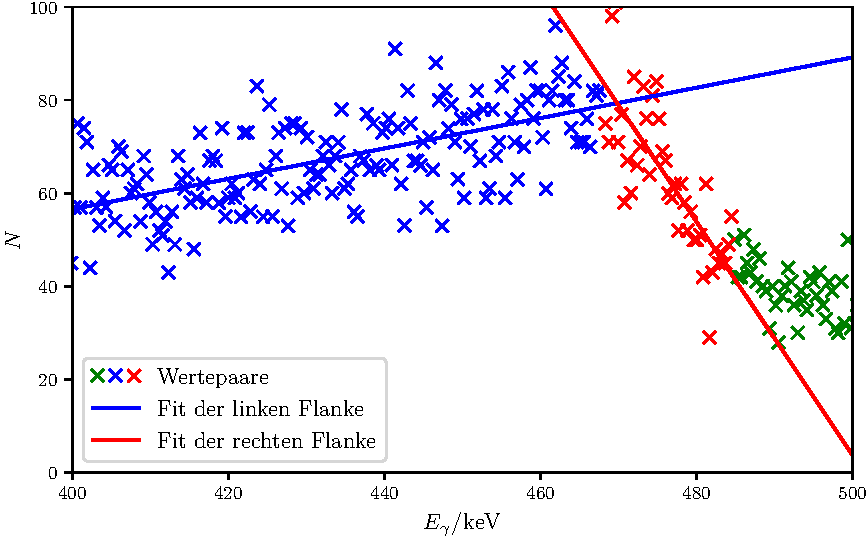
\includegraphics[width=\linewidth-60pt,height=\textheight-60pt,keepaspectratio]{content/images/Cs137Emax.pdf}
	\caption{Die Bestimmung der Position der Compton-Kante des $^{137}.{Cs}$-Strahlers. Die blauen Werte werden in die Ausgleichsrechnung der linken Flanke mit einbezogen, die roten in die der Rechten. Die grünen Werte werden in den Ausgleichsrechnungen nicht berücksichtigt.}
	\label{fig:Emax}
\end{figure}

\begin{table}
	\centering
	\caption{Die Parameter der gefitteten Geraden zur Bestimmung der Position der Compton-Kante des Spektrums von $^{137}.{Cs}$.}
	\label{tab:geraden2}
	\sisetup{table-format=1.2}
	\begin{tabular}{lS[table-format=2.2]@{${}\pm{}$}S[table-format=1.2]S[table-format=4.0]@{${}\pm{}$}S[table-format=3.0]}
		\toprule
		{} & \multicolumn{2}{c}{$m$} & \multicolumn{2}{c}{$n$} \\
		\midrule
		{linke Flanke}  & 0.33 & 0.04 &  -74 &  14 \\
		{rechte Flanke} & -2.5 & 0.4  & 1260 & 160 \\
		\bottomrule
	\end{tabular}

	\label{tab:geradenEmax}
\end{table}

\newpage
\noindent Es werden die Inhalte des Kontinuums und des Photopeaks ermittelt. Der Inhalt des Photopeaks berechnet sich nach Formel \eqref{eq:I_Gaus}. Die Anzahl der Ereignisse im Bereich des Compton-Kontinuums wird bestimmt, indem die Daten durch eine Ausgleichskurve nach Formel \eqref{eq:sigmadiff}, welche durch einen Streckungsfaktor $a$ und einen Achsenabschnitt $b$ ergänzt wurde, approximiert werden (vergleiche Abbildung \ref{fig:Comptonkontinuum}). Es ergeben sich die Parameter:
\begin{align*}
a	&= \SI{4.99(22)e32}{\kilo\electronvolt\per\metre\squared}\text{,}\\
b	&= \num{15.4(19)}\text{.}\\
\end{align*}
Die Integration der Kurve liefert den Inhalt des Kontinuums.
Es ergeben sich für die Inhalte die Werte:
\begin{align*}
I_.{Photo} 	 &= \num{1.62(3)e4}\text{,}\\
I_.{Compton} &= \num{5.95(7)e4}\text{.}\\
\end{align*} 
Das ergibt ein Verhältnis der Inhalte von:
\[
\frac{I_.{Compton}}{I_.{Photo}} = \num{3.67(7)}\text{.}
\]
Der theoretische Wert des Verhältnisses $V_.{theo}$ bestimmt sich mit dem Extinktionskoeffizienten des Photopeaks von $\SI{0.0075}{\per\centi\per\metre}$ und dem des Kontinuums von $\SI{0.37}{\per\centi\per\metre}$ gemäß Abbildung \ref{fig:Wirkungsquerschnitt}, sowie Formel \eqref{eq:Nd} zu: 
\[
V_.{theo} = \num{26.5(18)}\text{.}
\]

\begin{figure}
	\centering
	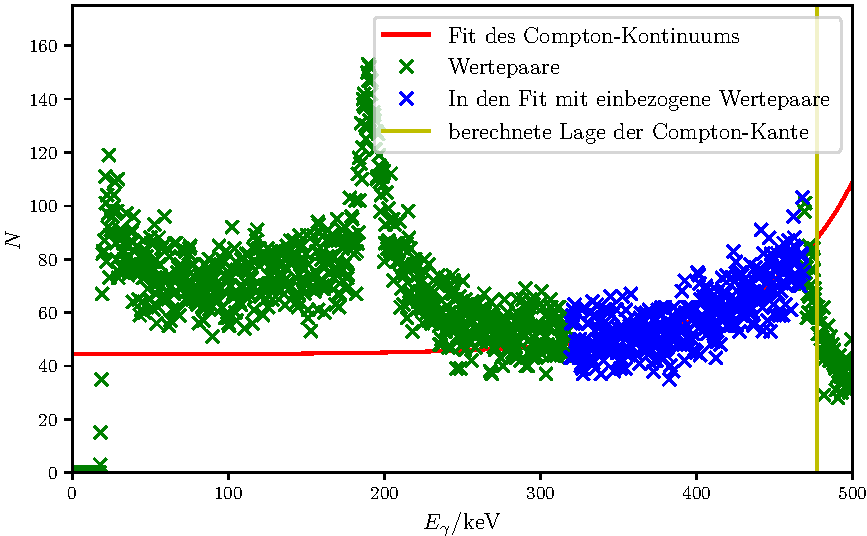
\includegraphics[width=\linewidth-60pt,height=\textheight-60pt,keepaspectratio]{content/images/Cs137Kon.pdf}
	\caption{Die Approximation des Compton-Kontinuums des $^{137}.{Cs}$-Strahlers.}
	\label{fig:Comptonkontinuum}
\end{figure}

\subsection{Bestimmung der Aktivität einer unbekannten Probe}

Es wird die Aktivität einer weiteren Probe bestimmt. Das Spektrum wird über eine Messzeit von $\SI{6312}{\second}$ aufgenommen und ist in Abbildung \ref{fig:Ba} zu sehen. Mit den Ergebnissen wird geklärt, ob es sich um eine $^{125}.{Sb}$- oder eine $^{133}.{Ba}$-Probe handelt.
Dazu werden die Peaks des Spektrums durch Formel \eqref{eq:gaussFit} approximiert. Die Parameter befinden sich in Tabelle \ref{tab:parameterBa}. Die bestimmten Energien werden mit der Literatur \cite{KHAZOV2011855} verglichen. Es ist zu erkennen, dass es sich bei der Probe um $^{133}.{Ba}$ handelt.\\
Gemäß Formel \eqref{eq:Q} wird die Aktivität ermittelt. Dabei wird $Z$ nach Formel \eqref{eq:I_Gaus} berechnet. Werden die Ergebnisse der Aktivitäten der Peaks mit einer Energie über $\SI{150}{\kilo\electronvolt}$ aus Tabelle \ref{tab:ABa} gemittelt, so ergibt sich eine mittlere Aktivität von:
\[
A_.{Ba} = \SI{1263(9)}{\becquerel}\text{.}
\]

\begin{figure}
	\centering
	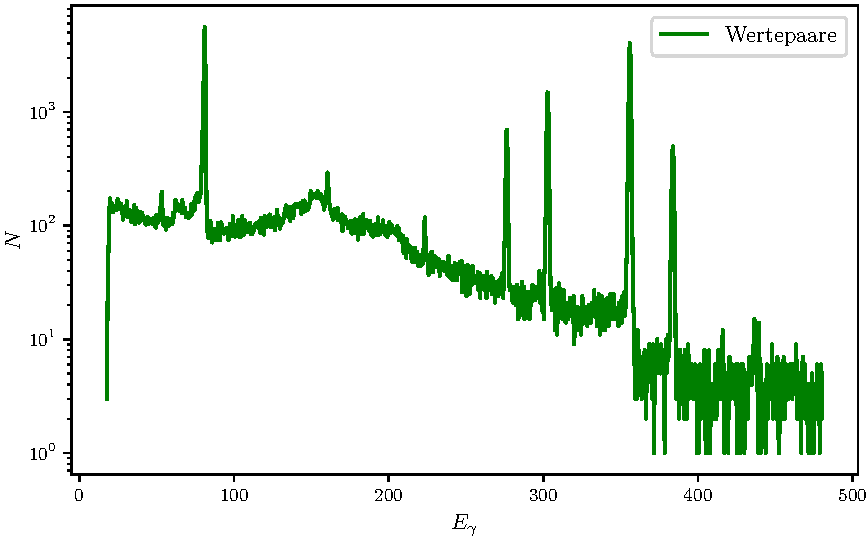
\includegraphics[width=\linewidth-60pt,height=\textheight-60pt,keepaspectratio]{content/images/D.pdf}
	\caption{Das Spektrum des Strahlers, bei einer Messzeit von $\SI{6312}{\second}$.}
	\label{fig:Ba}
\end{figure}

\begin{table}
	\centering
	\caption{Die Parameter der gefitteten Peaks des Spektrums mit den ermittelten Energien. Zudem die aus der Literatur entnommenen Energien $E_\gamma^\text{lit}$ \cite{KHAZOV2011855}.}
	\label{tab:D}
	\sisetup{table-format=1.2}
	\begin{tabular}{S[table-format=3.3]@{${}\pm{}$}S[table-format=1.3]S[table-format=1.3]@{${}\pm{}$}S[table-format=1.3]S[table-format=4.0]@{${}\pm{}$}S[table-format=3.0]S[table-format=3.1]@{${}\pm{}$}S[table-format=2.1]S[table-format=3.2]@{${}\pm{}$}S[table-format=1.2]S[table-format=3.4]@{${}\pm{}$}S[table-format=1.4]}
		\toprule
		\multicolumn{2}{c}{$b$} & \multicolumn{2}{c}{$\sigma$} & \multicolumn{2}{c}{$a$} & \multicolumn{2}{c}{$c$} & \multicolumn{2}{c}{$E_\gamma/\si{\kilo\electronvolt}$} & \multicolumn{2}{c}{$E_\gamma^{\text{lit}}/\si{\kilo\electronvolt}$} \\
		\midrule
		208.63  & 0.04  & 1.06  & 0.04  & 5596 & 164 & 222  & 56  & 81.02 & 0.05 & 80.9979 & 0.0011 \\
		693.562 & 0.011 & 1.311 & 0.011 &  709 &   6 & 27.0 & 0.7 & 276.41 & 0.04 & 276.3989 & 0.0012 \\
		759.247 & 0.011 & 1.407 & 0.012 & 1501 &  11 & 23   & 4   & 302.87 & 0.03 & 302.8508 & 0.0005 \\
		891.107 & 0.008 & 1.505 & 0.008 & 4000 &  17 & 19   & 6   & 356.00 & 0.03 & 356.0129 & 0.0007 \\
		960.125 & 0.019 & 1.639 & 0.021 &  493 &   5 & 5.8  & 1.9 & 383.81 & 0.03 & 383.8485 & 0.0012 \\
		\bottomrule
	\end{tabular}

	\label{tab:parameterBa}
\end{table}

\begin{table}
	\centering
	\caption{Die berechneten Peakinhalte $Z$, die mit den Vollenergienachweiswahrscheinlichkeiten $Q$ berechneten Aktivitäten $A$,  sowie die berechneten Energien $E_\gamma$.  Zudem die aus der Literatur entnommenen Energien $E_\gamma^\text{lit}$ und Emissions-Wahrscheinlichkeiten $W$ \cite{KHAZOV2011855}.}
	\label{tab:D2}
	\sisetup{table-format=1.2}
	\begin{tabular}{S[table-format=3.2]@{${}\pm{}$}S[table-format=1.2]S[table-format=3.4]@{${}\pm{}$}S[table-format=1.4]S[table-format=2.2]@{${}\pm{}$}S[table-format=1.2]S[table-format=5.0]@{${}\pm{}$}S[table-format=3.0]S[table-format=1.3]@{${}\pm{}$}S[table-format=1.3]S[table-format=4.0]@{${}\pm{}$}S[table-format=2.0]}
		\toprule
		\multicolumn{2}{c}{$E_\gamma/\si{\kilo\electronvolt}$} & \multicolumn{2}{c}{$E_\gamma^{\text{lit}}/\si{\kilo\electronvolt}$} & \multicolumn{2}{c}{$W/\si{\percent}$} & \multicolumn{2}{c}{$Z$} & \multicolumn{2}{c}{$Q$} & \multicolumn{2}{c}{$A/\si{\becquerel}$} \\
		\midrule
		81.02 & 0.05  & 80.9979  & 0.0011 & 32.95 & 0.33 & 14932 & 526 & 0.90  & 0.05  &  511 & 31 \\
		276.41 & 0.04 & 276.3989 & 0.0012 & 7.16  & 0.05 &  2329 &  18 & 0.257 & 0.006 & 1290 & 32 \\
		302.87 & 0.03 & 302.8508 & 0.0005 & 18.34 & 0.13 &  5294 &  43 & 0.234 & 0.005 & 1258 & 30 \\
		356.00 & 0.03 & 356.0129 & 0.0007 & 62.05 & 0.19 & 15093 &  78 & 0.198 & 0.004 & 1250 & 25 \\
		383.81 & 0.03 & 383.8485 & 0.0012 & 8.94  & 0.07 &  2024 &  26 & 0.183 & 0.004 & 1257 & 29 \\
		\bottomrule
	\end{tabular}

	\label{tab:ABa}
\end{table}

\subsection{Identifizierung der aktiven Nuklide in einer Zerfallsreihe}

Anhand des Spektrums eines unbekannten Strahlers wird versucht einige aktive Nuklide einer Zerfallsreihe zu bestimmen. Das Spektrum des Strahlers wurde über einen Zeitraum von $\SI{4489}{\second}$ aufgenommen und ist in Abbildung \ref{fig:SpektrumUnbekannt} zu sehen. Es wird wie bei der Untersuchung von $^{133}.{Ba}$ vorgegangen. Die Parameter der Ausgleichsrechnung befinden sich in Tabelle \ref{tab:parameterUnbekannt}. Durch Vergleich der berechneten Energien mit der Literatur \cite{V18} lassen sich $^{234}.{Th}$, $^{226}.{Ra}$, $^{214}.{Pb}$ und $^{214}.{Bi}$ als aktive Nuklide identifizieren. Die Werte für $Z$ und $A$ werden analog zu $^{133}.{Ba}$ berechnet und befinden sich in Tabelle \ref{tab:AUnbekannt}

\begin{figure}
	\centering
	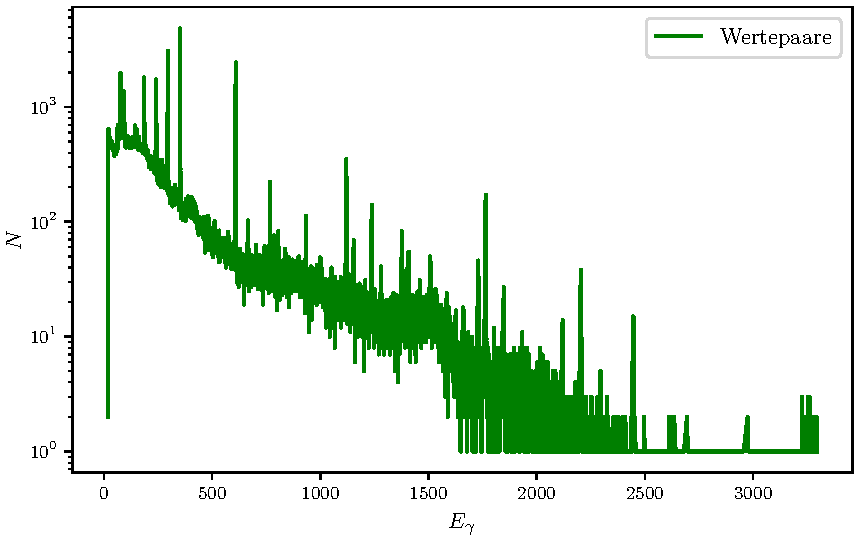
\includegraphics[width=\linewidth-60pt,height=\textheight-60pt,keepaspectratio]{content/images/unbekannt.pdf}
	\caption{Das aufgenommene Spektrum einer unbekannten Probe, bei einer Messzeit von $\SI{4489}{\second}$.}
	\label{fig:SpektrumUnbekannt}
\end{figure}

\begin{table}
	\centering
	\caption{Die Parameter der gefitteten Peaks des unbekannten Spektrums mit den ermittelten Energien.}
	\label{tab:unbekannt}
	\sisetup{table-format=1.2}
	\begin{tabular}{r@{${}\pm{}$}lr@{${}\pm{}$}lr@{${}\pm{}$}lr@{${}\pm{}$}lr@{${}\pm{}$}l}
		\toprule
		\multicolumn{2}{c}{$b$} & \multicolumn{2}{c}{$\sigma$} & \multicolumn{2}{c}{$a$} & \multicolumn{2}{c}{$c$} & \multicolumn{2}{c}{$E_\gamma/\si{\kilo\electronvolt}$} \\
		\midrule
		237.41   & 0.14  & 1.20  & 0.14  & 810    & 80   & 589   & 24  & 92.62   & 0.07 \\
		469.349  & 0.025 & 1.375 & 0.028 & 1449   & 24   & 423   & 8   & 186.07  & 0.04 \\
		608.182  & 0.026 & 1.310 & 0.027 & 1478   & 26   & 273   & 8   & 242.01  & 0.04 \\
		740.278  & 0.010 & 1.371 & 0.010 & 2982   & 18   & 194   & 6   & 295.23  & 0.03 \\
		880.925  & 0.012 & 1.500 & 0.013 & 4620   & 40   & 150   & 9   & 351.90  & 0.03 \\
		1519.301 & 0.021 & 2.089 & 0.022 & 2478   & 22   & 52    & 7   & 609.11  & 0.03 \\
		1913.96  & 0.08  & 2.54  & 0.09  & 188    & 5    & 36.1  & 1.6 & 768.13  & 0.04 \\
		2325.40  & 0.15  & 3.04  & 0.16  & 81     & 4    & 28.3  & 1.1 & 933.90  & 0.07 \\
		2787.46  & 0.05  & 3.09  & 0.05  & 334    & 5    & 21.5  & 1.3 & 1120.07 & 0.04 \\
		3426.36  & 0.26  & 3.63  & 0.28  & 59     & 4    & 16.8  & 1.3 & 1377.49 & 0.11 \\
		3485.8   & 0.4   & 3.5   & 0.6   & 19.1   & 2.0  & 16.0  & 1.7 & 1401.45 & 0.14 \\
		3752.41  & 0.29  & 3.9   & 0.4   & 34.1   & 2.3  & 14.4  & 0.9 & 1508.87 & 0.13 \\
		4299.91  & 0.24  & 4.74  & 0.26  & 32.2   & 1.5  & 3.9   & 0.6 & 1729.46 & 0.11 \\
		4386.30  & 0.12  & 4.71  & 0.13  & 163    & 4    & 3.9   & 1.2 & 1764.27 & 0.08 \\
		5477.59  & 0.20  & 5.72  & 0.21  & 33.8   & 1.1  & 1.2   & 0.4 & 2203.97 & 0.12 \\
		\bottomrule
	\end{tabular}

	\label{tab:parameterUnbekannt}
\end{table}

\begin{table}
	\centering
	\caption{Die zu den aus der Literatur entnommenen Energien $E_\gamma^\text{lit}$ und Emissions-Wahrscheinlichkeiten $W$ \cite{V18} zugeordneten Energien, sowie die zugehörigen Elemente.}
	\label{tab:unbekannt2}
	\sisetup{table-format=1.2}
	\begin{tabular}{cr@{${}\pm{}$}lS[table-format=4.0]S[table-format=2.0]}
		\toprule
		{Element} & \multicolumn{2}{c}{$E_\gamma/\si{\kilo\electronvolt}$} & {$E_\gamma^{\text{lit}}/\si{\kilo\electronvolt}$} & {$W/\si{\percent}$} \\
		\midrule
		{$^{234}.{Th}$} & 92.62   & 0.07 &   93 &  4 \\
		{$^{226}.{Ra}$} & 186.07  & 0.04 &  186 &  4 \\
		{$^{214}.{Pb}$} & 242.01  & 0.04 &  242 &  4 \\
		{$^{214}.{Pb}$} & 295.23  & 0.03 &  295 & 19 \\
		{$^{214}.{Pb}$} & 351.90  & 0.03 &  352 & 36 \\
		{$^{214}.{Bi}$} & 609.11  & 0.03 &  609 & 47 \\
		{$^{214}.{Bi}$} & 768.13  & 0.04 &  769 &  5 \\
		{$^{214}.{Bi}$} & 933.90  & 0.07 &  935 &  3 \\
		{$^{214}.{Bi}$} & 1120.07 & 0.04 & 1120 & 17 \\
		{$^{214}.{Bi}$} & 1377.49 & 0.11 & 1378 &  5 \\
		{$^{214}.{Bi}$} & 1401.45 & 0.14 & 1400 &  4 \\
		{$^{214}.{Bi}$} & 1508.87 & 0.13 & 1509 &  2 \\
		{$^{214}.{Bi}$} & 1729.46 & 0.11 & 1728 &  3 \\
		{$^{214}.{Bi}$} & 1764.27 & 0.08 & 1764 & 17 \\
		{$^{214}.{Bi}$} & 2203.97 & 0.12 & 2204 &  5 \\
		\bottomrule
	\end{tabular}

	\label{tab:AUnbekannt}
\end{table}

